%%%%%%%%%%%%%%%%%%%%%%%%%%%%%%%%%%%%%%%%%%%%%%%%%%%%%%%%%%% Author - Varad Meru
%% tex source file for ML Homeworks
%%%%%%%%%%%%%%%%%%%%%%%%%%%%%%%%%%%%%%%%%%%%%%%%%%%%%%%%%
\documentclass[a4paper, 11pt]{article}

\usepackage[margin=1in]{geometry} % changes the margin
\usepackage{lipsum} % adds random text to check the formatting
\usepackage{hyperref} % adds hyperlink
\usepackage[framed,numbered,autolinebreaks,useliterate]{mcode}
\usepackage{subfigure}
\usepackage{amsmath}
\usepackage{graphicx}
\usepackage{enumerate}

\renewcommand{\thefootnote}{\fnsymbol{footnote}} % Changes the format of the footnotes superscripts

%%%%%%%%%%%%%%%%%%%%%%%%%%%%%%%%%%%%%%%%%%%%%%%%%%%%%%%%%
\begin{document}

\begin{noindent}
\large\textbf{Week 9} \hfill \textbf{Varad Meru} \\
\normalsize CS 273a - Introduction to Machine Learning (Winter '15)\footnote{\href{http://sli.ics.uci.edu/Classes/2015W-273a}{Website: http://sli.ics.uci.edu/Classes/2015W-273a}} \hfill Student \# 26648958 \\
Prof. Alex Ihler \hfill Due Date: 03/10/2015
\end{noindent}	
\noindent\makebox[\linewidth]{\rule{\textwidth}{0.4pt}}

%%%%%%%%%%%%%%%%%%%%%%%%%%%%%%%%%%%%%%%%%%%%%%%%%%%%%%%%%
%%%%%%%%%%%%%%%%%%%%%%%%%%%%%%%%%%%%%%%%%%%%%%%%%%%%%%%%%
\begin{center}
\textbf{\Large{Homework 5}\footnote{Questions available at \href{http://sli.ics.uci.edu/Classes/2015W-273a?action=download\&upname=HW5.pdf}{http://sli.ics.uci.edu/Classes/2015W-273a?action=download\&upname=HW5.pdf}}\footnote{All the figures and listing numbers are auto-referred.}}\\
\end{center}
\vspace{-25pt}

%%%%%%%%%%%%%%%%%%%%%%%%%%%%%%%%%%%%%%%%%%%%%%%%%%%%%%%%%
%%%%%%%%%%%%%%%%%%%%%%%%%%%%%%%%%%%%%%%%%%%%%%%%%%%%%%%%%
%%%%%%%%%%%%%%%%%%%%%%%%%%%%%%%%%%%%%%%%%%%%%%%%%%%%%%%%%
\section*{Problem 1: Basics of Clustering}
\begin{enumerate}[(a)]
\item The dataset is loaded in Matlab, as shown in \autoref{lst:scatter} and \autoref{fig:sctr}
\vspace{-20pt}
\begin{lstlisting}[caption={Loading Data},label={lst:scatter},numbers=left,escapeinside={@}{@}]
% Problem a
iris=load('data/iris.txt');     % load the text file
X = iris(:,1:2);       % features are other columns
features = char('Sepal length','Sepal width','Petal length','Petal width','Species');
features_short = char('SL','SW','PL','PW','SP');
whos

f = figure;
scatter(X(:,1), X(:,2), 'filled');
saveas(f,'scatter.png','png');
\end{lstlisting}
\item The \autoref{lst:kmeans1} shows the code listing for problem of k-means for different values of k and initialization methods. The \autoref{fig:kmeans1} shows the plot of the created clusters.
\vspace{-20pt}
\begin{lstlisting}[caption={K-Means on iris dataset for different values of k and initialization methods.},label={lst:kmeans1},numbers=left,escapeinside={@}{@}]
%% Problem b
k = 5;
[z,c,sumd] = kmeans(X,k);
[z1,c1,sumd1] = kmeans(X,k,'k++');

f = figure;
plotClassify2D([],X,z);
saveas(f,'kmeans_k_5_simple.png', 'png');

f = figure;
plotClassify2D([],X,z1);
saveas(f,'kmeans_k_5_kpp.png', 'png');

k = 20;
[z,c,sumd] = kmeans(X,k);
[z1,c1,sumd1] = kmeans(X,k,'k++');

f = figure;
plotClassify2D([],X,z);
saveas(f,'kmeans_k_20_simple.png', 'png');

f = figure;
plotClassify2D([],X,z1);
saveas(f,'kmeans_k_20_kpp.png', 'png');
\end{lstlisting}

\item The \autoref{lst:kmeans2} shows the code listing for problem of k-means for different values of k and initialization methods. The \autoref{fig:kmeans2} shows the plot of the created clusters.
\vspace{-20pt}
\begin{lstlisting}[caption={Agglomerative clustering on iris dataset for different values of k and linkage methods.},label={lst:kmeans2},numbers=left,escapeinside={@}{@}]
%% Problem c
k = 5;
Z = linkage(X,'single');
c = cluster(Z,'maxclust',k);
f = figure;
plotClassify2D([],X,c);
saveas(f,'linkage_single_5.png', 'png');
f = figure;
dendrogram(Z)
saveas(f,'dendogram_5.png', 'png');

Z = linkage(X,'complete');
c = cluster(Z,'maxclust',k);
f = figure;
plotClassify2D([],X,c);
saveas(f,'linkage_complete_5.png', 'png');

k = 20;
Z = linkage(X,'single');
c = cluster(Z,'maxclust',k);
f = figure;
plotClassify2D([],X,c);
saveas(f,'linkage_single_20.png', 'png');
f = figure;
dendrogram(Z)
saveas(f,'dendogram_20.png', 'png');

Z = linkage(X,'complete');
c = cluster(Z,'maxclust',k);
f = figure;
plotClassify2D([],X,c);
saveas(f,'linkage_complete_20.png', 'png');
\end{lstlisting}
\item The EM Gaussian mixture model is run with 5 and 20 components, as shown in \autoref{lst:kmeans3}. The generated clusters can be seen in \autoref{fig:kmeans3}.
\begin{lstlisting}[caption={The EM Gaussian mixture model for 5 and 20 components.},label={lst:kmeans3},numbers=left,escapeinside={@}{@}]
%% Problem d
k = 5;
[zx,Tx,softx,llx] = emCluster(X,k);
f = figure;
plotClassify2D([],X,zx);
saveas(f,'emgm_5.png', 'png');

k = 20;
[zx,Tx,softx,llx] = emCluster(X,k);
f = figure;
plotClassify2D([],X,zx);
saveas(f,'emgm_20.png', 'png');
\end{lstlisting}
All the three clustering mechanisms bring different properties and have different usecases. The Agglomerative clustering has a simple architecture and works well for simple and small dataset. EM Gaussian mixture models are well suited for fuzzy nature of dataset where a data might not be strictly associated with any cluster. Traditional means as a low computational complexity compared to others, $O(nkt)$, where $n$ is the number of datapoints, $k$ is the number of clusters and $t$ is the number of iterations. And thus, it can be computed repeatedly to search for a good configuration. With all the methods, `k-means ++' gave good results.
\end{enumerate}

\begin{figure}
\centering
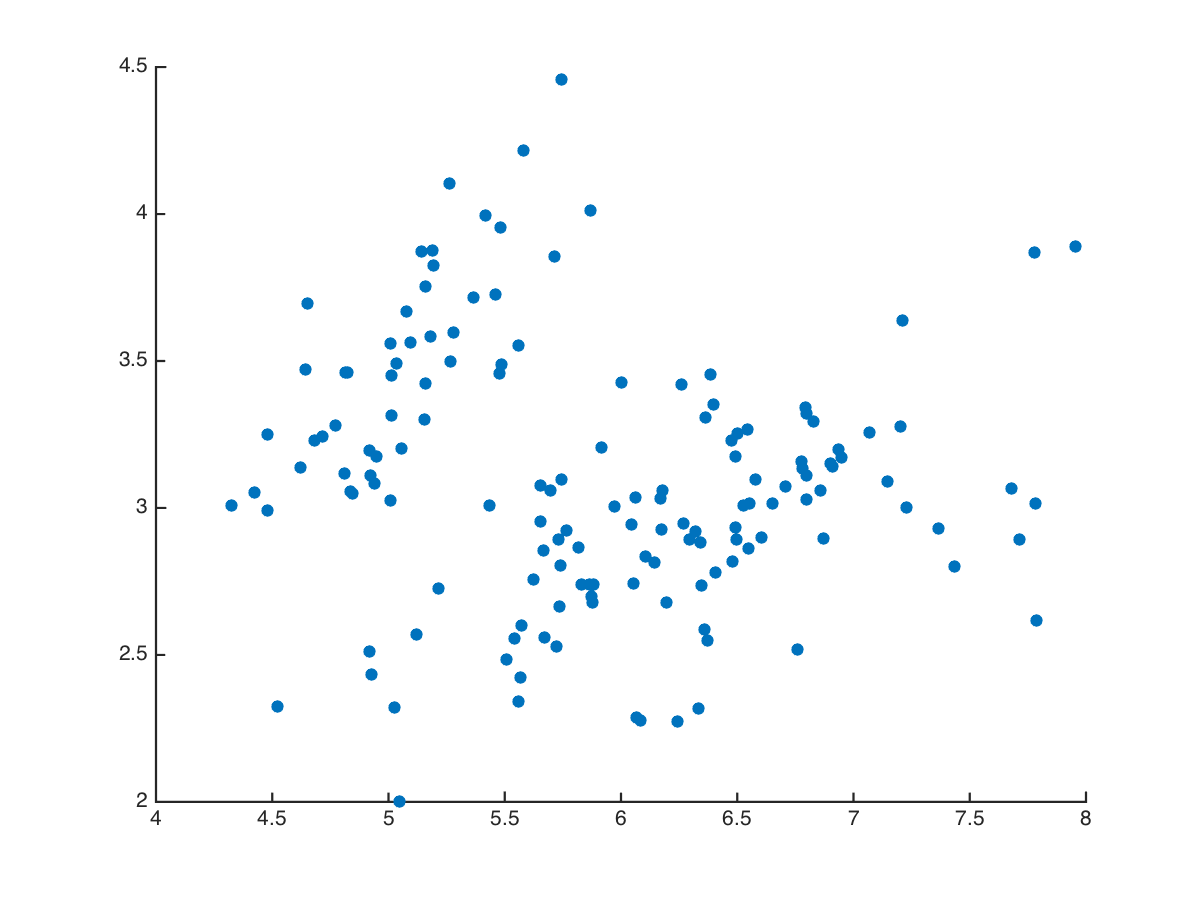
\includegraphics[scale=0.50]{scatter.png}
\caption[]{Data Loaded}
\label{fig:sctr}
\end{figure}


\begin{figure}
\centering
\subfigure[\mcode{k=5} Random Initialisation]{
    \label{fig:subfig1}
    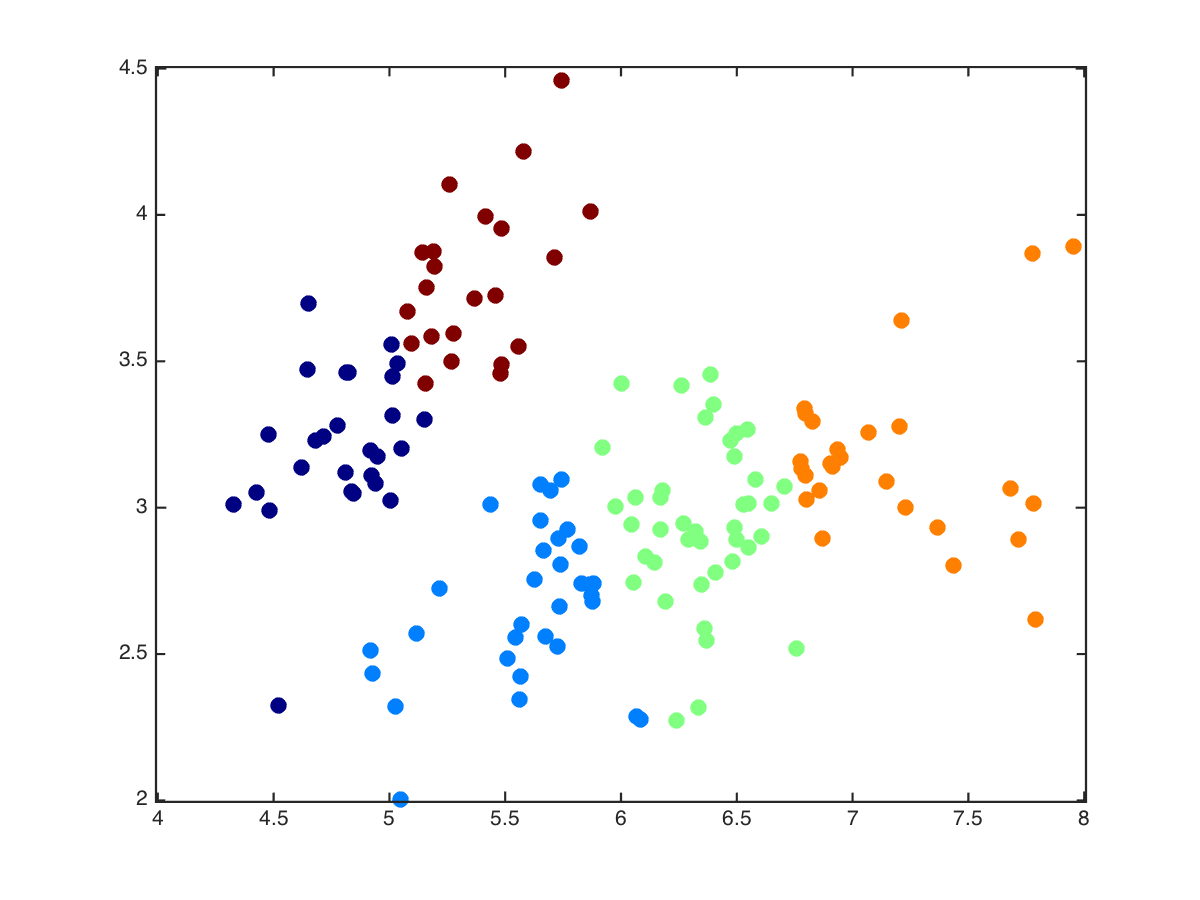
\includegraphics[scale=0.35]{kmeans1.png}
}
\subfigure[\mcode{k=5} Initialisation using K-Means++]{
    \label{fig:subfig2}
    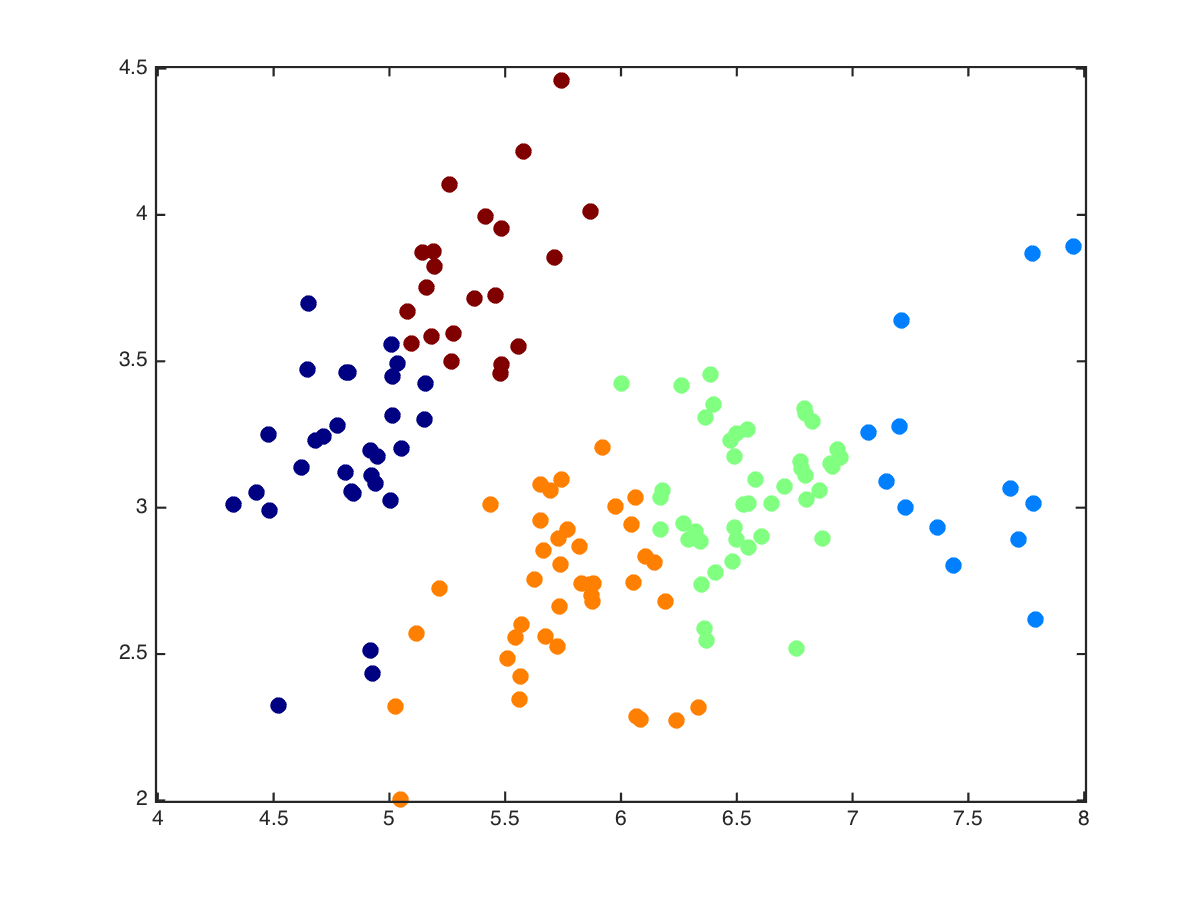
\includegraphics[scale=0.35]{kmeans2.png}
}
\subfigure[\mcode{k=20} Random Initialisation]{
    \label{fig:subfig2}
    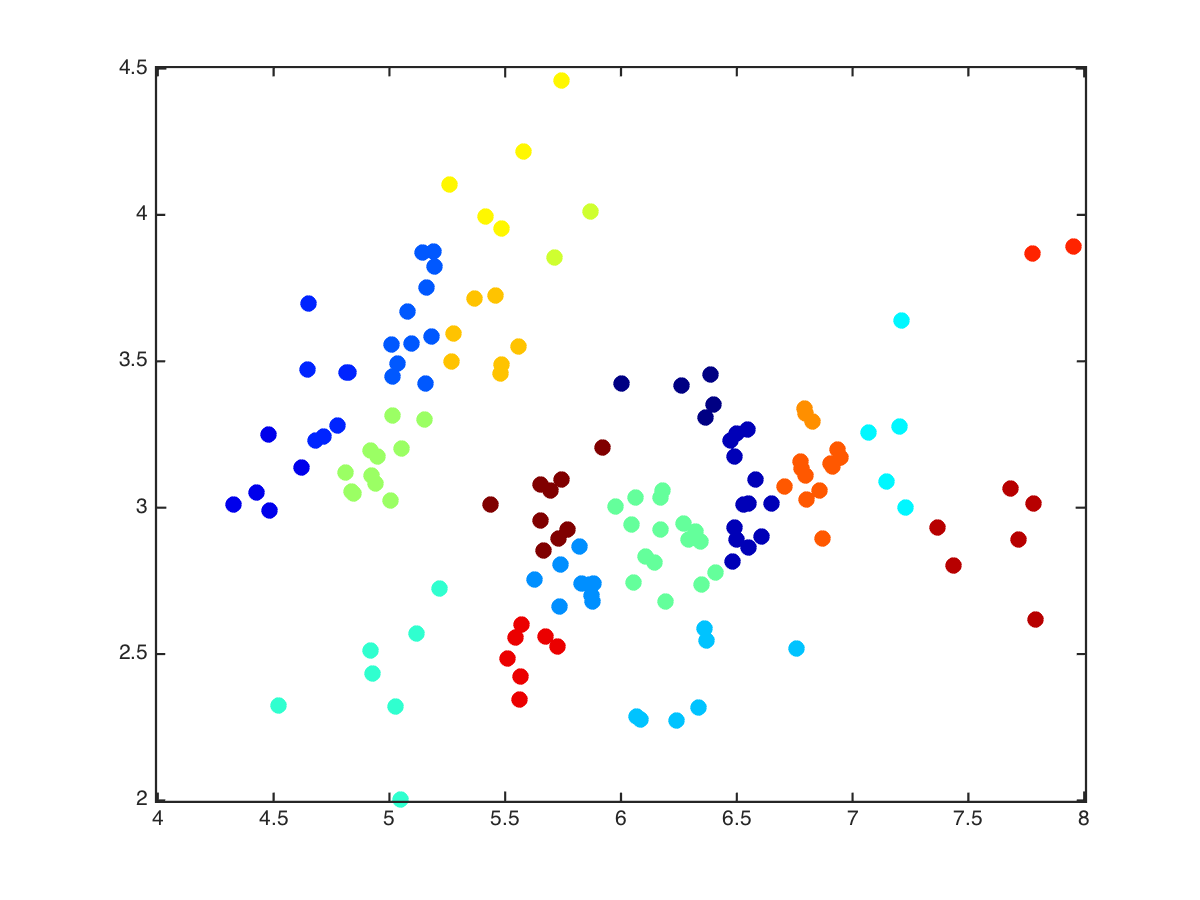
\includegraphics[scale=0.35]{kmeans3.png}
}
\subfigure[\mcode{k=20} Initialisation using K-Means++]{
    \label{fig:subfig2}
    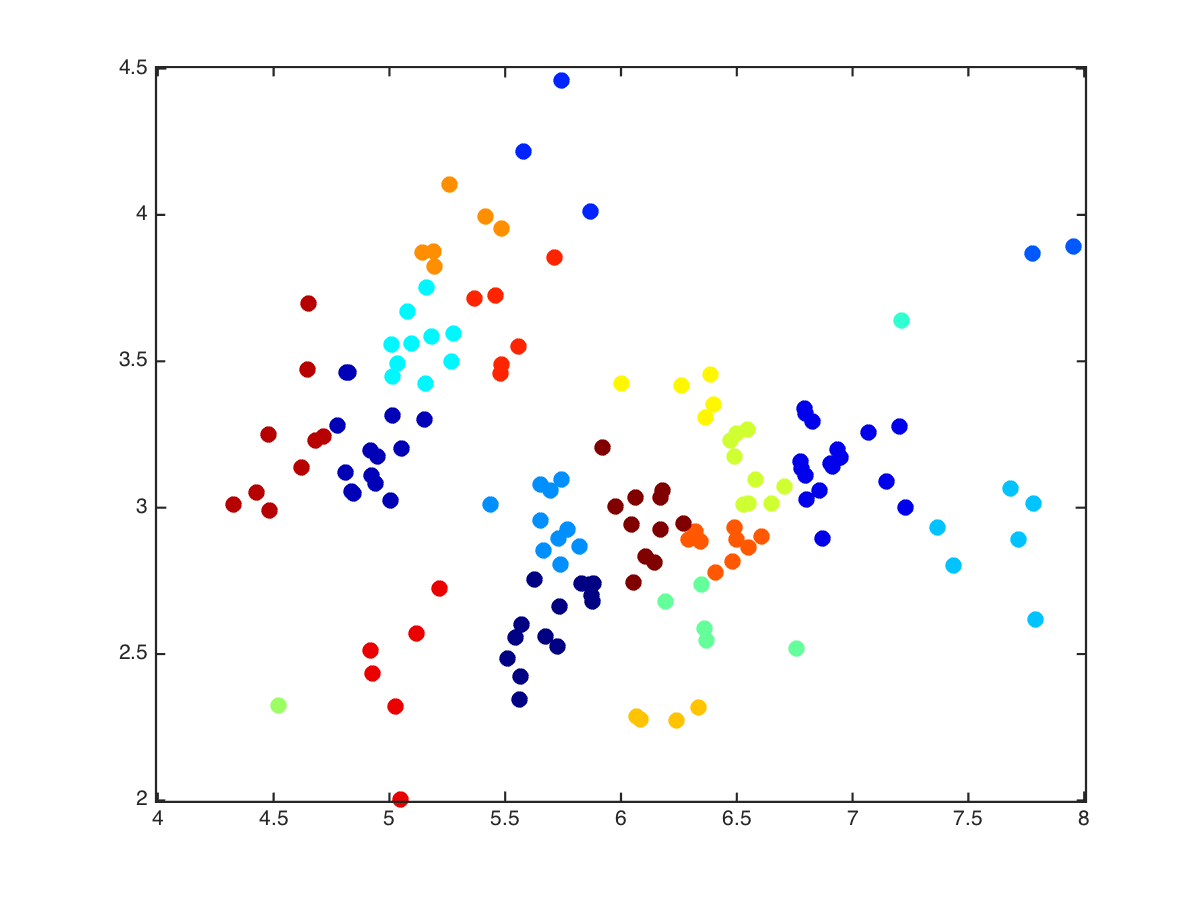
\includegraphics[scale=0.35]{kmeans4.png}
}
\caption[]{Various runs of K-Means different values of k and initialization methods}
\label{fig:kmeans1}
\end{figure}

\begin{figure}
\centering
\subfigure[Complete Dendrogram of the created clusters]{
    \label{fig:subfig1}
    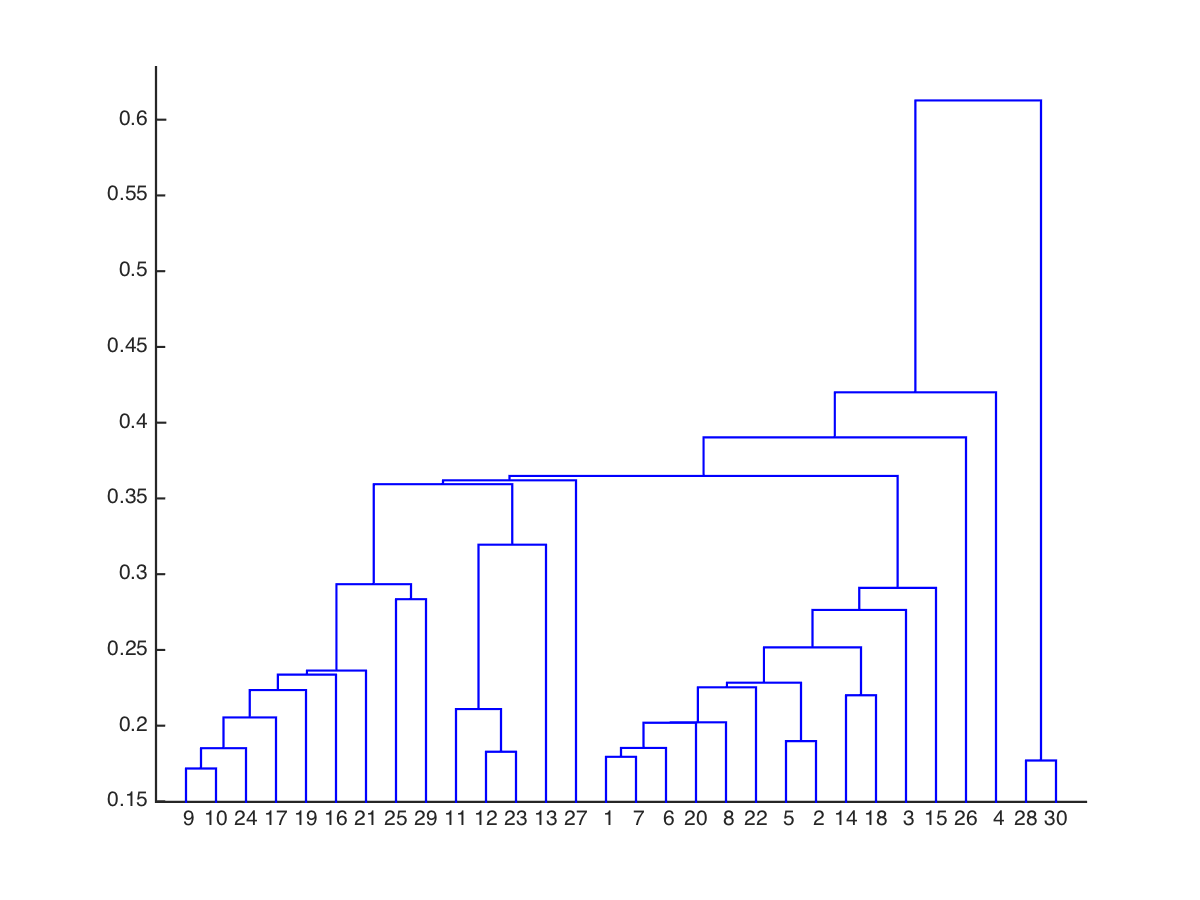
\includegraphics[scale=0.40]{dendogram_5.png}
}
\subfigure[\mcode{k=5} Linkage method = single]{
    \label{fig:subfig2}
    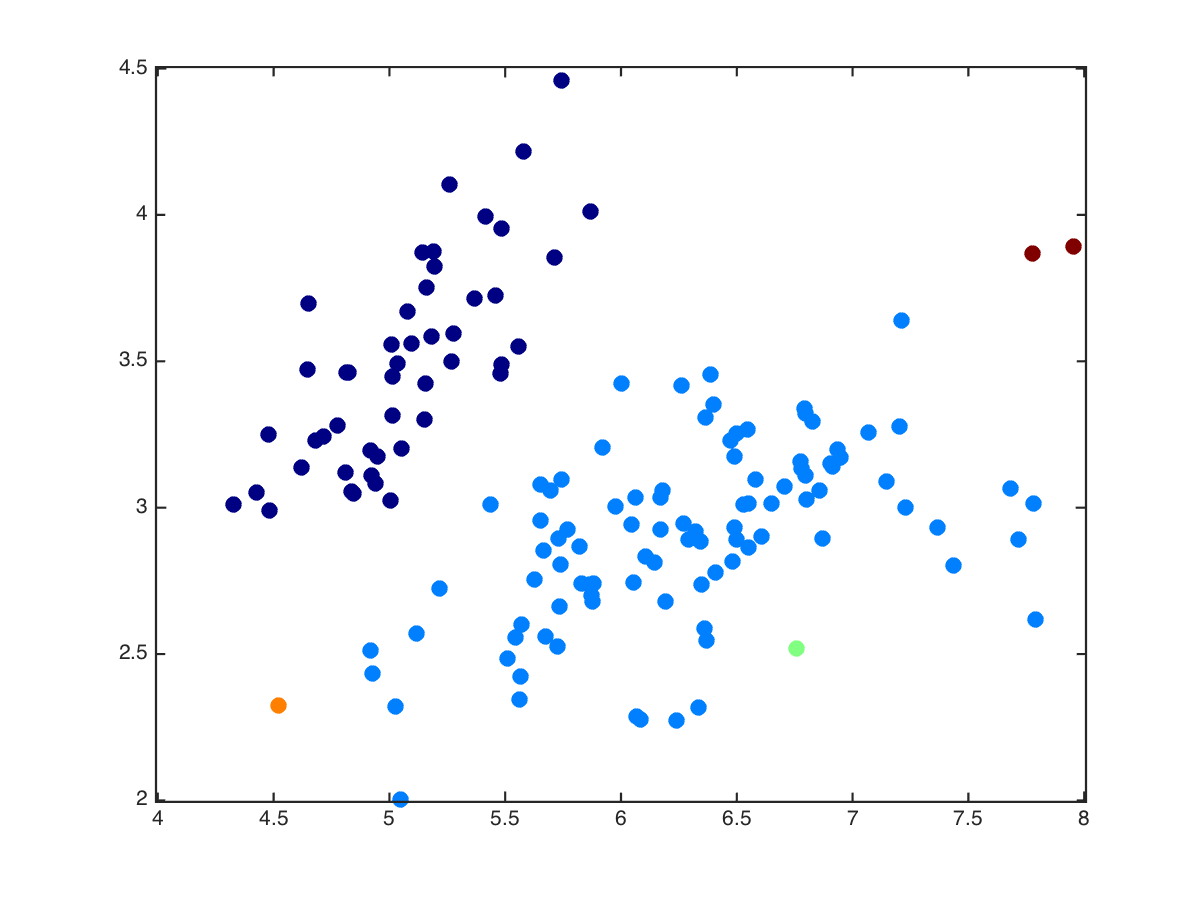
\includegraphics[scale=0.35]{linkage_single_5.png}
}
\subfigure[\mcode{k=5} Linkage method = complete]{
    \label{fig:subfig2}
    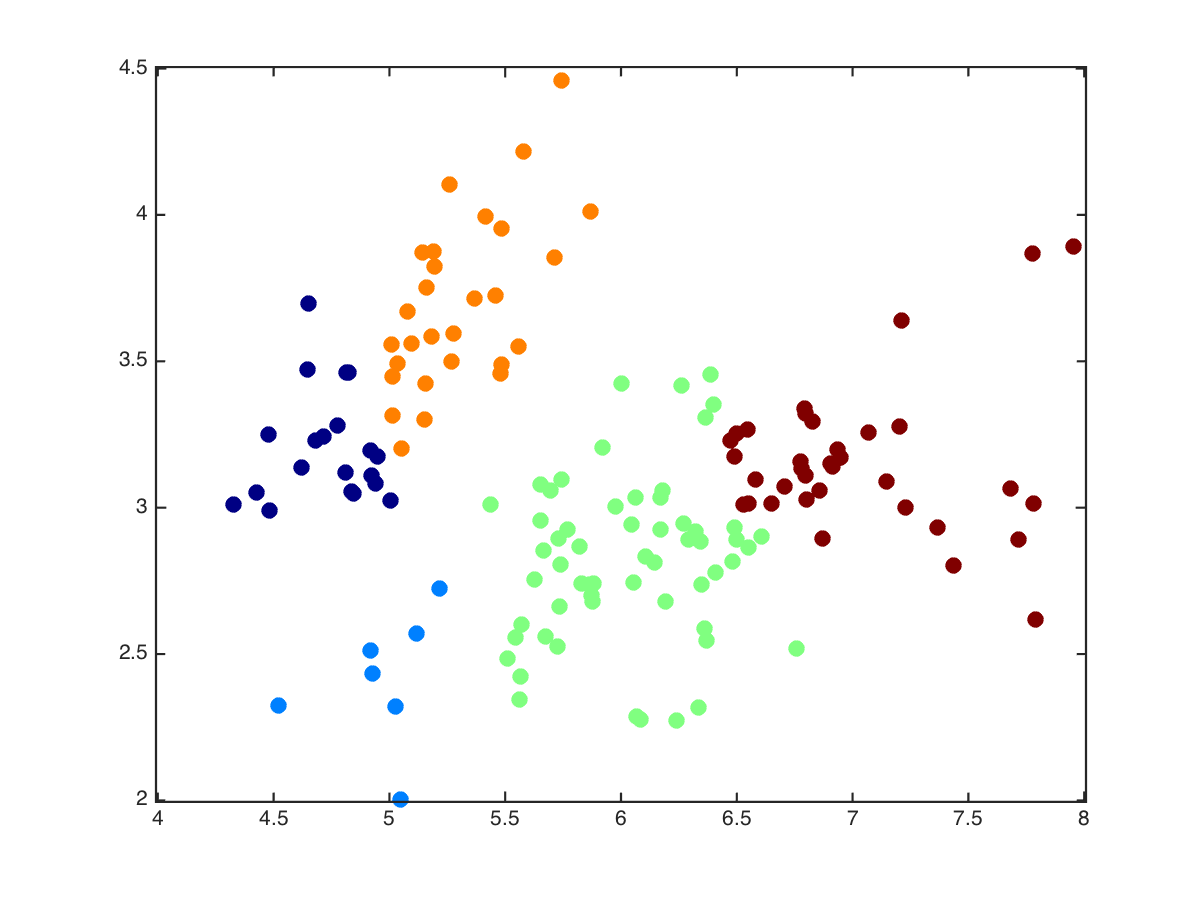
\includegraphics[scale=0.35]{linkage_complete_5.png}
}
\subfigure[\mcode{k=20} Linkage method = single]{
    \label{fig:subfig2}
    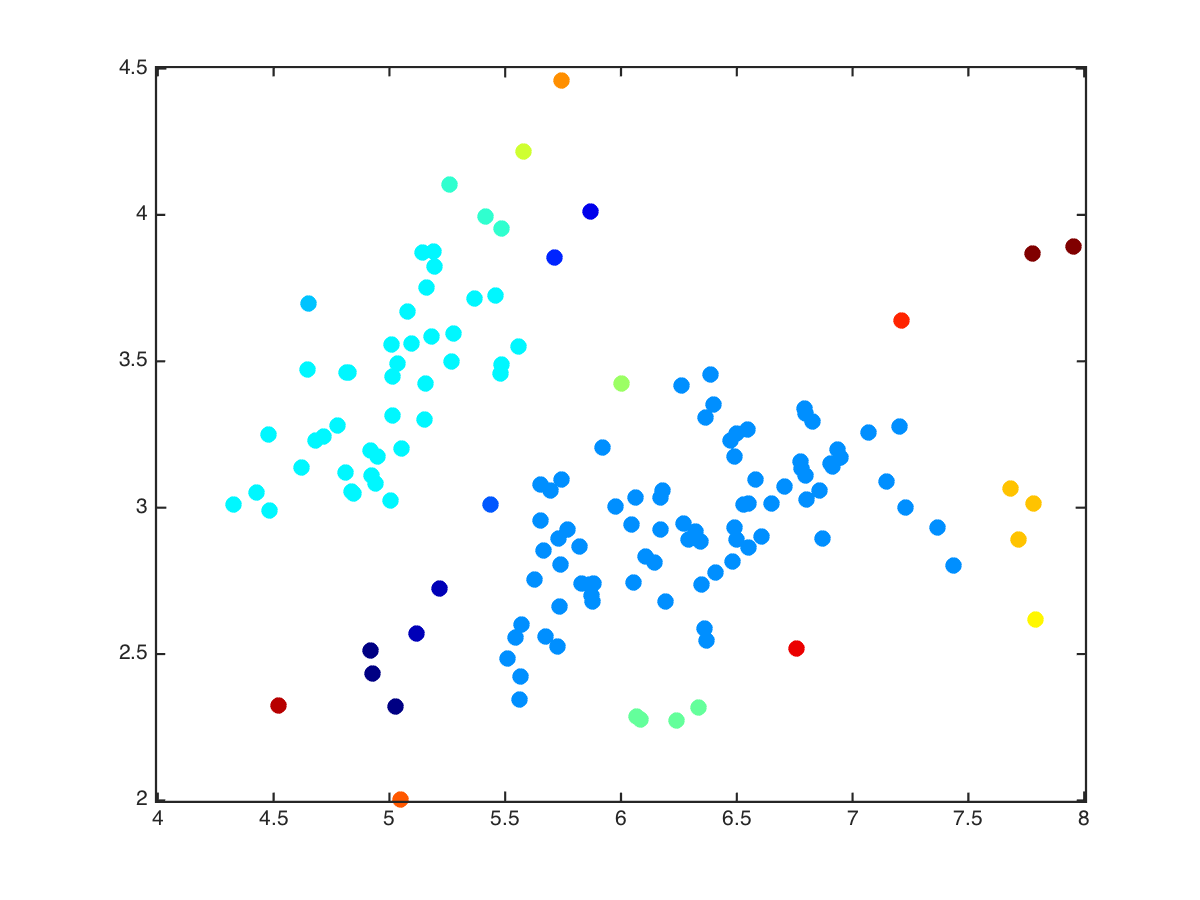
\includegraphics[scale=0.35]{linkage_single_20.png}
}
\subfigure[\mcode{k=20} Linkage method = complete]{
    \label{fig:subfig2}
    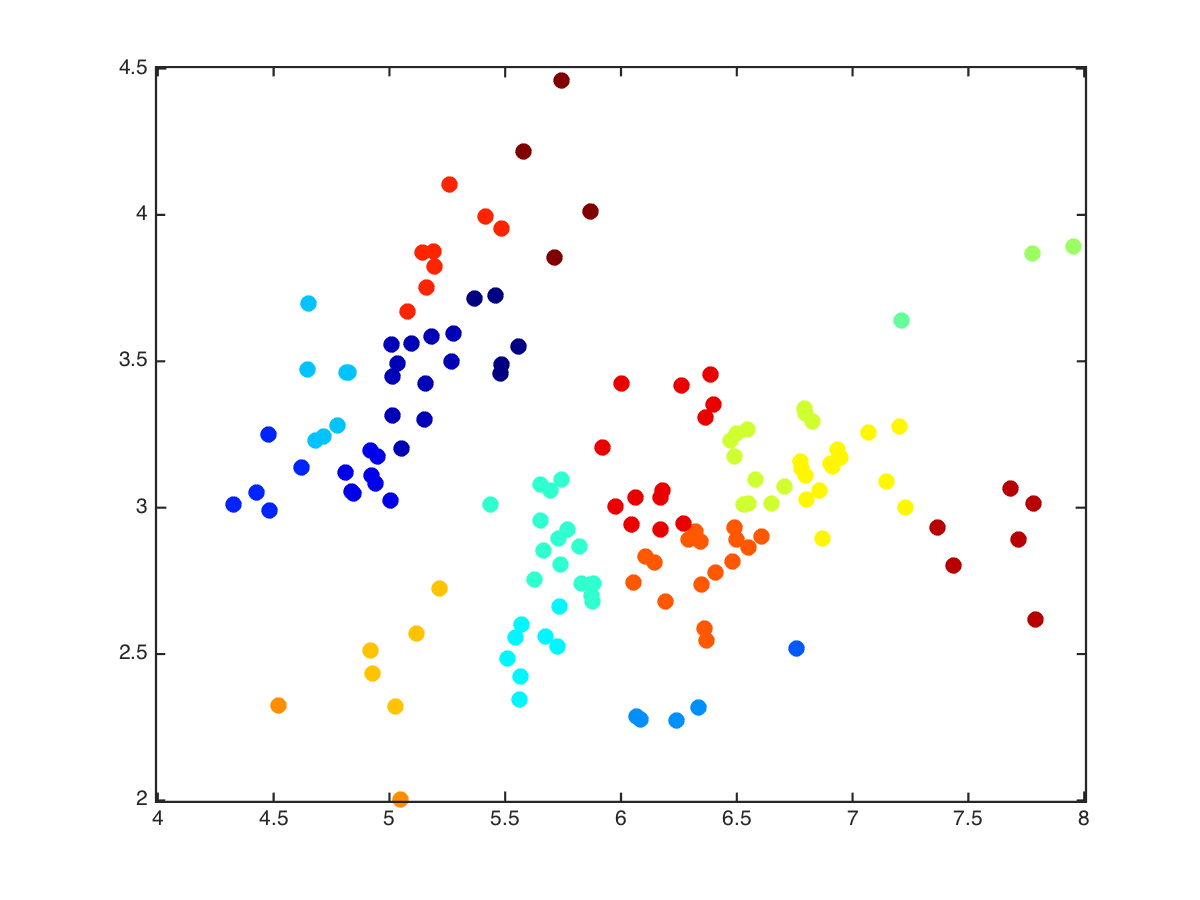
\includegraphics[scale=0.35]{linkage_complete_20.png}
}
\caption[]{Various runs of Agglomerative clustering with different values of k and linkage methods}
\label{fig:kmeans2}
\end{figure}

\begin{figure}
\centering
\subfigure[\mcode{k=5} Random Initialisation]{
    \label{fig:subfig1}
    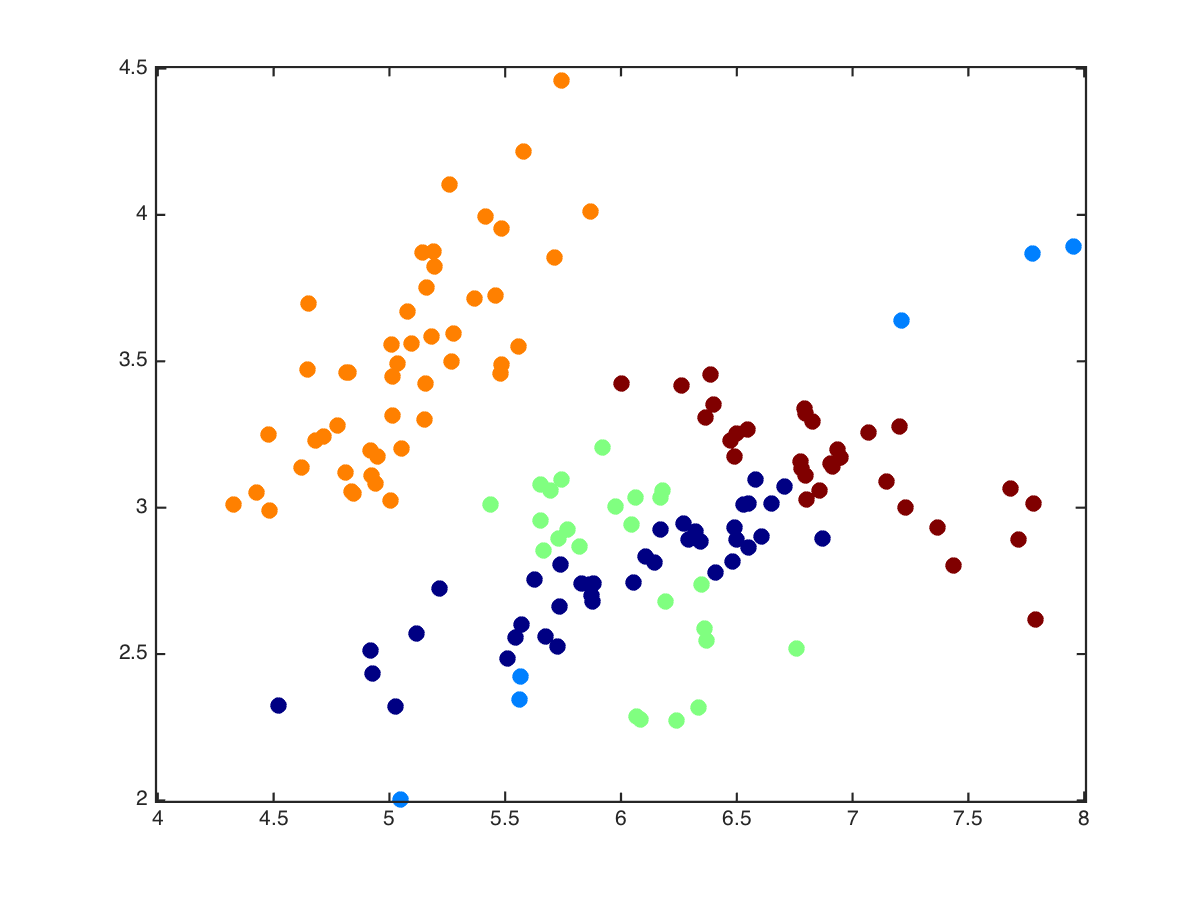
\includegraphics[scale=0.35]{emgm_5.png}
}
\subfigure[\mcode{k=5} Initialisation using K-Means++]{
    \label{fig:subfig2}
    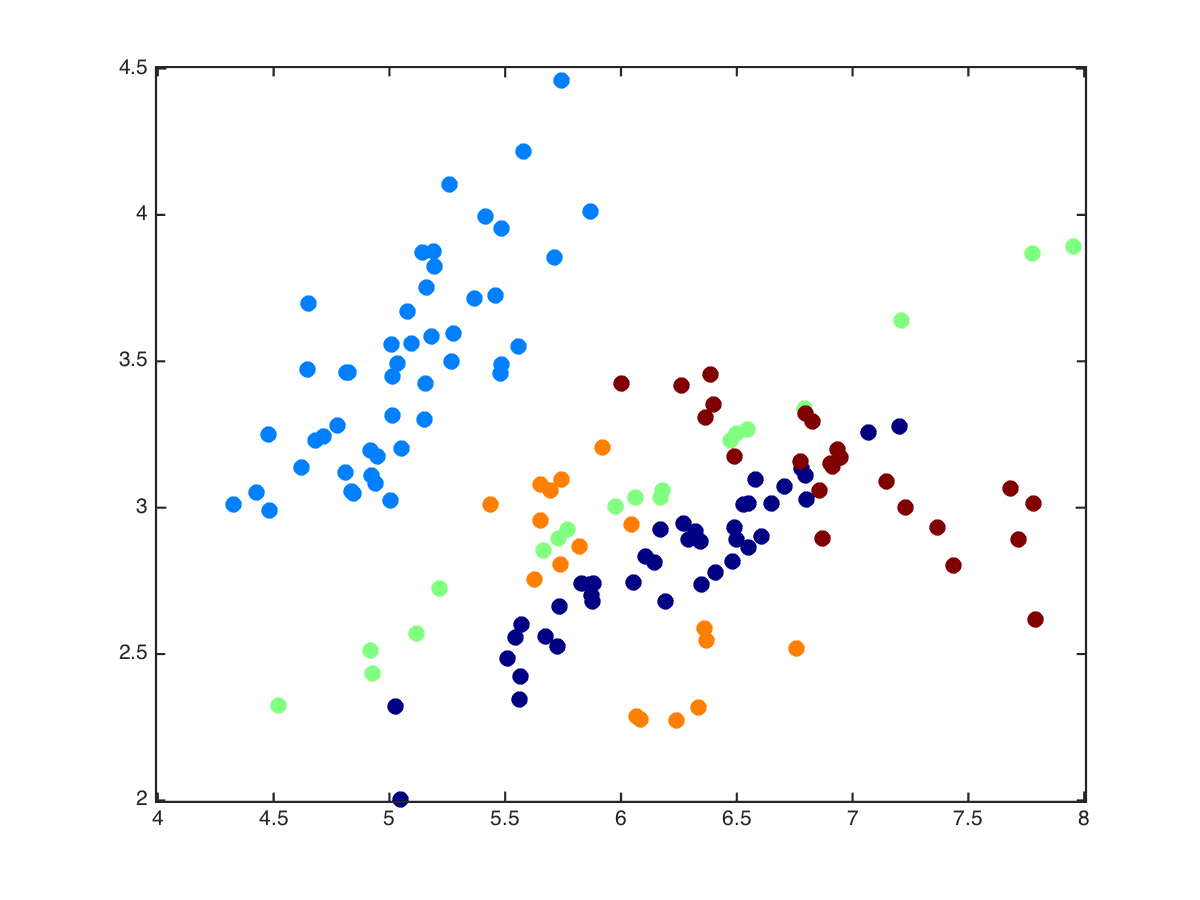
\includegraphics[scale=0.35]{emgm_5_kpp.png}
}
\subfigure[\mcode{k=20} Initialisation using K-Means++]{
    \label{fig:subfig2}
    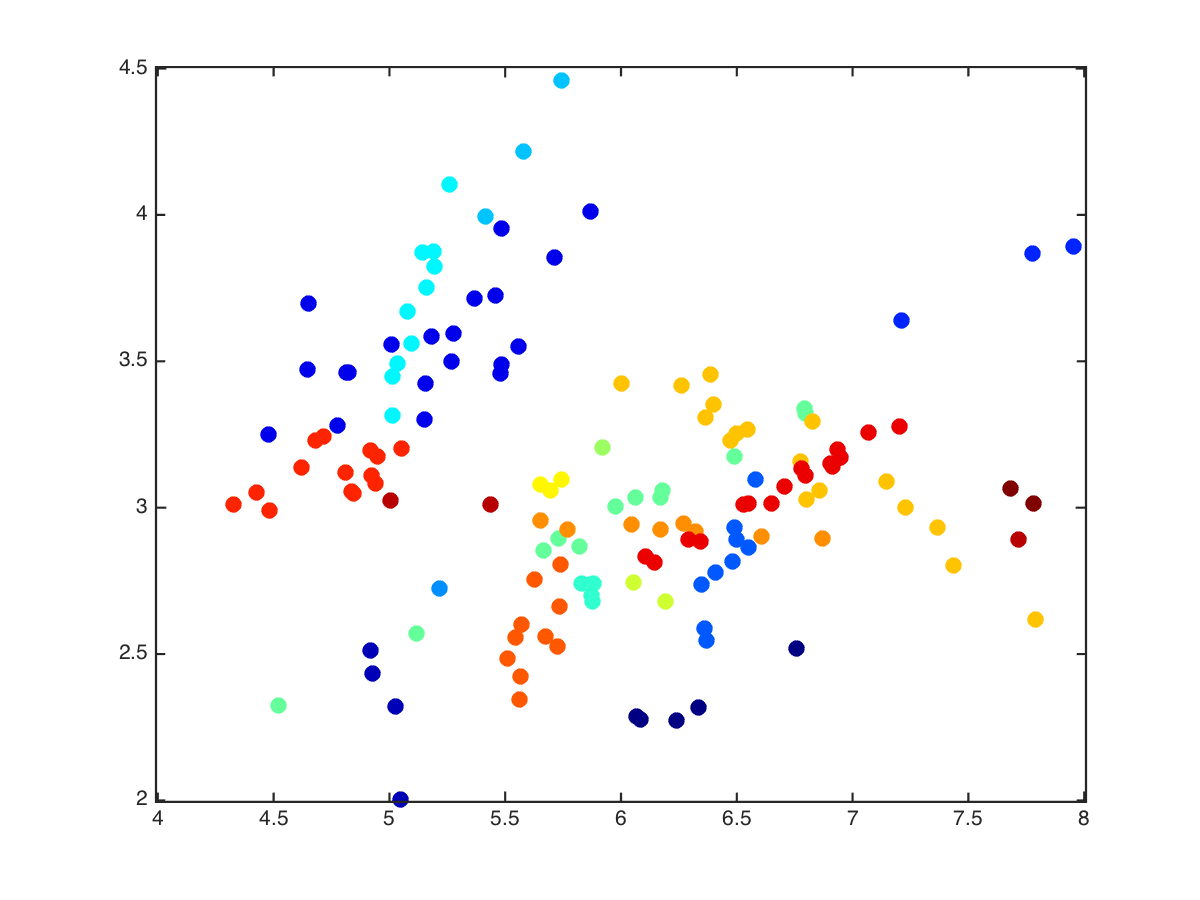
\includegraphics[scale=0.35]{emgm_20.png}
}
\subfigure[\mcode{k=20} Initialisation using K-Means++]{
    \label{fig:subfig2}
    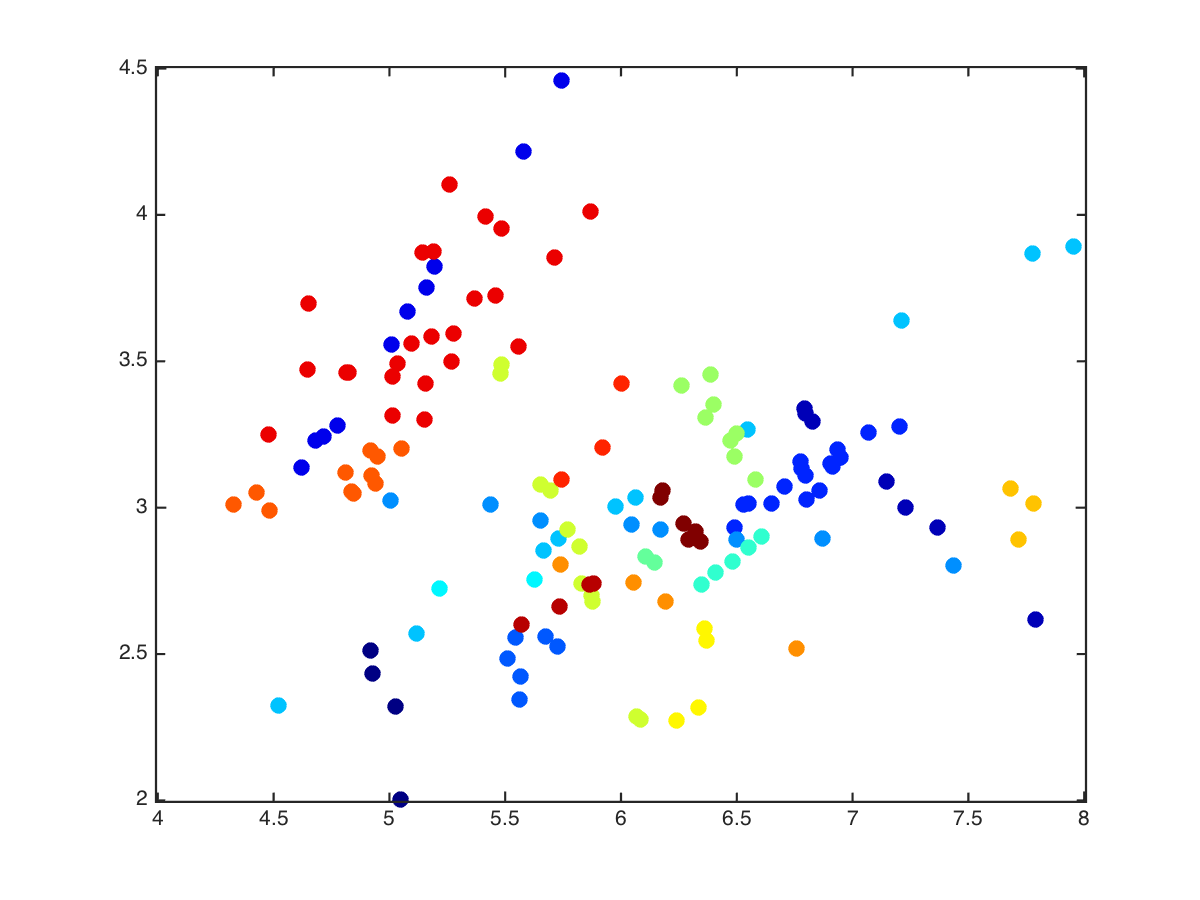
\includegraphics[scale=0.35]{emgm_20_kpp.png}
}
\caption[]{EM Gaussian mixture model with different values of k and initialization methods}
\label{fig:kmeans3}
\end{figure}

\pagebreak

%%%%%%%%%%%%%%%%%%%%%%%%%%%%%%%%%%%%%%%%%%%%%%%%%%%%%%%%%
%%%%%%%%%%%%%%%%%%%%%%%%%%%%%%%%%%%%%%%%%%%%%%%%%%%%%%%%%
\section*{Problem 2: K Means Clustering on Text}
\begin{enumerate}[(a)]
\item The clusters are computed using \mcode{kmeans()} method provided by Matlab and the code that produces can be seen in \autoref{lst:kmeans4}.
\vspace{-20pt}
\begin{lstlisting}[caption={K-means on textual data with \mcode{k=20} and for part (b), the number of runs = 20},label={lst:kmeans4},numbers=left,escapeinside={@}{@}]
%% Problem (a, b)
k = 20;
[z,c,sumd] = kmeans(Xn,k);
disp(sumd)
disp('--------------')
for i=1:20;
    [z1,c1,sumd1] = kmeans(Xn,k);
    disp(sumd1)
    if sumd1 < sumd
        z = z1;
        c = c1;
        sumd = sumd1;
    end;
end;
display('Minimum-sumd')
disp(sumd)
%{
    2.4211
--------------
    2.0789
    2.1009
    2.0453
    2.0625
    2.0861
    2.4494
    2.0615
    2.0709
    2.0646
    2.1144
    2.0098
    2.0530
    2.4806
    2.0479
    2.0587
    2.0811
    2.4695
    1.9865
    2.4891
    2.0573

Minimum-sumd
    1.9865
%}
\end{lstlisting}
\item \autoref{lst:kmeans4} shows 20 runs of K-Means on the textual data and I got the best value of the cost function to be \mcode{sumd = 1.9865}.

\item For counting the document accusation with clusters, I use a function called \mcode{count_unique()}, and it gives the output as given in \autoref{lst:kmeansuniq} as well as the bar graph of the distribution can be seen at \autoref{fig:bar1}. For the second part of the question, I used a slight modification of the original code given in the homework to populate the document terms. The code and the output can be seen in \autoref{lst:kmeansdocs}.
\begin{lstlisting}[caption={The number of documents for each cluster},label={lst:kmeansuniq},numbers=left,escapeinside={@}{@}]
>> [uniques,numUnique] = count_unique(z)
>> [uniques,numUnique]
ans =
     1    21
     2    45
     3     4
     4     2
     5     7
     6     8
     7    69
     8     3
     9    10
    10     2
    11     2
    12     1
    13     1
    14     3
    15     1
    16     1
    17    15
    18     2
    19     3
    20     2
\end{lstlisting}
\vspace{-20pt}
\begin{lstlisting}[caption={The ``Most-Likely'' terms in the 20 clusters},label={lst:kmeansdocs},numbers=left,escapeinside={@}{@}]
%% Problem (c) - 2
for i =1:size(c, 1);
    [sorted,order] = sort( c(i,:), 2, 'descend');
    fprintf('Doc %d: ',i);
    fprintf('%s ', vocab{order(1:10)});
    fprintf('\n');
end;
%{
Doc 1: times square millennium city 2000 night 000 eve york midnight 
Doc 2: team game season coach games players league play going win 
Doc 3: archbishop york bishop cardinal sports church began column american close 
Doc 4: america boat team zealand cup nippon gilmour challengers round true 
Doc 5: book century marks amp war week finds lives school boy 
Doc 6: yeltsin putin russia russian president power political kremlin chechnya russians 
Doc 7: city american national president 000 home millennium end political going 
Doc 8: fireworks island city midnight celebration lot millennium hour calls celebrations 
Doc 9: y2k koskinen system problems saturday 2000 reported computers friday officials 
Doc 10: tutsi hutu rwanda burundi ethnic country experts africa van 1994 
Doc 11: texas arkansas yards line offensive game season sacks games defensive 
Doc 12: test end houston 000 0101 0102 100 1900 1900s 1968 
Doc 13: cats beijing owners police association called carry chinese eat eating 
Doc 14: hijackers hostages pakistan burger told government indian india passengers killed 
Doc 15: sports angeles began brooklyn column los seen young eye game 
Doc 16: economy government putin system america businesses country economic president russia 
Doc 17: 2000 computer internet government systems york problem problems news city 
Doc 18: lakers jackson game star phil players record conference practice monday 
Doc 19: news atlanta constitution journal service moved cox y2k cnn millennium 
Doc 20: buses authority diesel natural gas plan mta city york hybrid 
%}
\end{lstlisting}

\begin{figure}
\centering
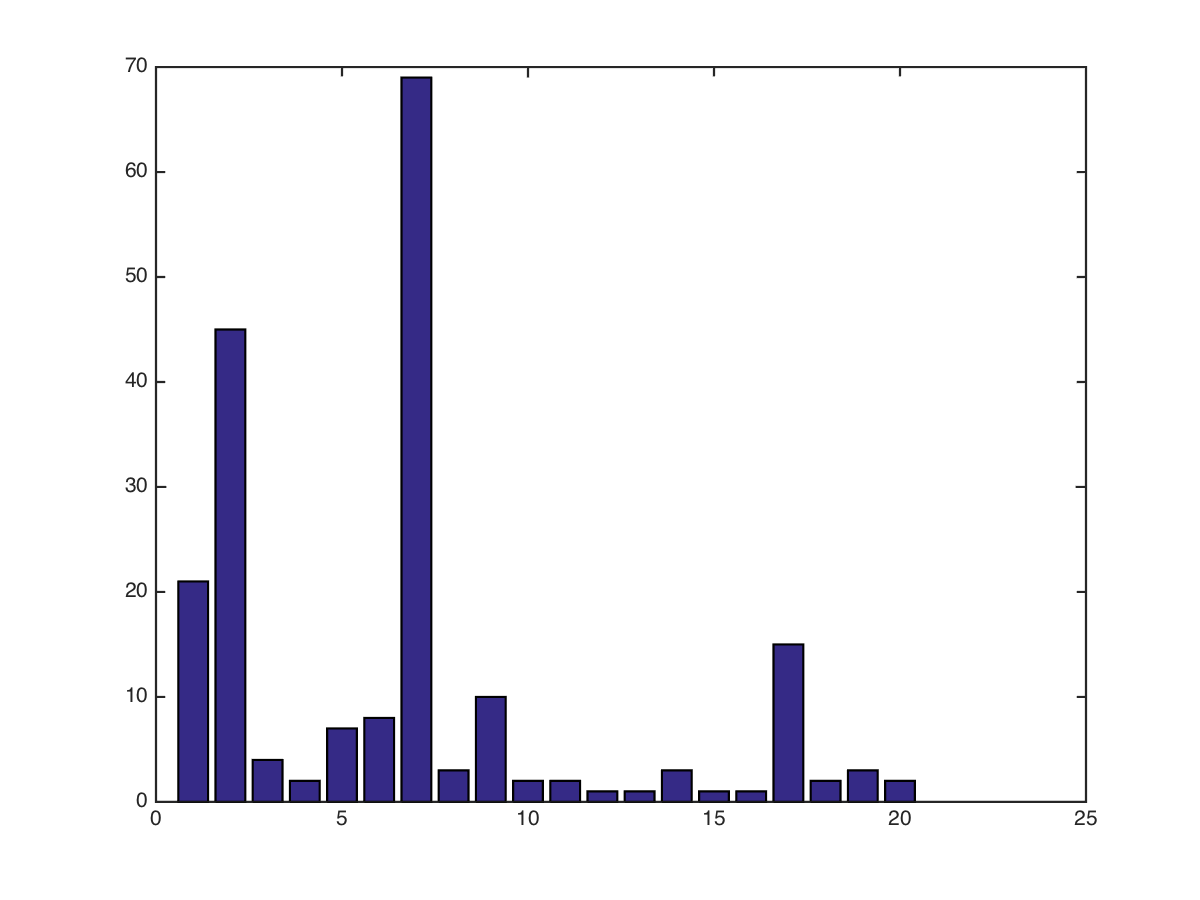
\includegraphics[scale=0.7]{bar1.png}
\caption[]{Distribution of the documents spread across \mcode{k=20} clusters.}
\label{fig:bar1}
\end{figure}
\item A
\end{enumerate}

%%%%%%%%%%%%%%%%%%%%%%%%%%%%%%%%%%%%%%%%%%%%%%%%%%%%%%%%%
%%%%%%%%%%%%%%%%%%%%%%%%%%%%%%%%%%%%%%%%%%%%%%%%%%%%%%%%%
\section*{Problem 3: Eigen Faces}
\begin{enumerate}[(a)]
\item Loading Eigen Faces Data, as can be seen in \autoref{lst:loadface}. Also see \autoref{fig:bar2}%\autoref{lst:face} and in the attached \autoref{fig:bar1}
\vspace{-20pt}
\begin{lstlisting}[caption={Loading Face Dataset},label={lst:loadface},numbers=left,escapeinside={@}{@}]
clc;close all;clear all;
rand('seed',0);
X = load('data/faces.txt'); % load face dataset
\end{lstlisting}

\item Normalisng the dataset.
\vspace{-20pt}
\begin{lstlisting}[caption={Normalizing},label={lst:loadface2},numbers=left,escapeinside={@}{@}]
%% Faces A
mu = mean(X);
X0 = bsxfun(@minus,X,mu);
size(mu);

%{
ans =
     1   576
%}
\end{lstlisting}

\end{enumerate}
\begin{figure}
\centering
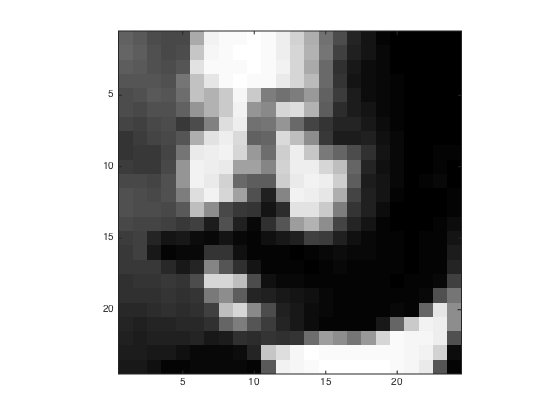
\includegraphics[scale=0.7]{face.png}
\caption[]{Face sample.}
\label{fig:bar2}
\end{figure}

%%%%%%%%%%%%%%%%%%%%%%%%%%%%%%%%%%%%%%%%%%%%%%%%%%%%%%%%%
%%%%%%%%%%%%%%%%%%%%%%%%%%%%%%%%%%%%%%%%%%%%%%%%%%%%%%%%%
\end{document}
%%%%%%%%%%%%%%%%%%%%%%%%%%%%%%%%%%%%%%%%%%%%%%%%%%%%%%%%%
%%%%%%%%%%%%%%%%%%%%%%%That's all folks%%%%%%%%%%%%%%%%%%%%%%%%%%%
%%%%%%%%%%%%%%%%%%%%%%%%%%%%%%%%%%%%%%%%%%%%%%%%%%%%%%%%%
\iffalse
\begin{figure}
\centering
\subfigure[Puzzle 1]{
    \label{fig:subfig1}
    \includegraphics[scale=0.30]{g1.png}
}
\subfigure[Puzzle 2]{
    \label{fig:subfig2}
    \includegraphics[scale=0.30]{g2.png}
}
\caption[Running Various Experiments]{Running Various Experiments. The three bars are for Brute Force, I-Consistency and I-Consistency with MRV search. All the times given are in Seconds}
\label{fig:rungraphs}
\end{figure}

\begin{figure}
\centering
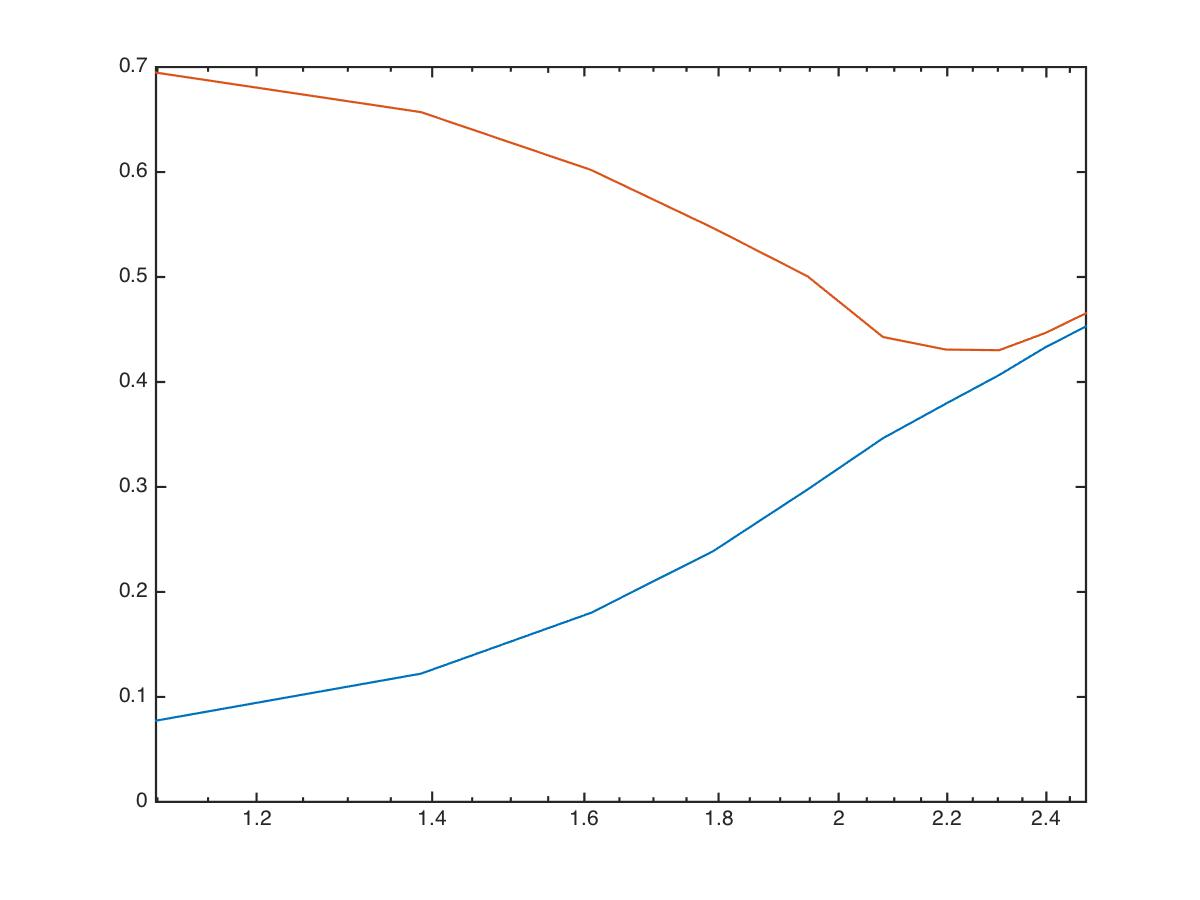
\includegraphics[scale=0.25]{minParent.jpg}
\caption[]{Text Here}
\label{fig:lr2}
\end{figure}

\begin{lstlisting}[caption={Plotting the scatter plot},label={lst:scatter},numbers=left,escapeinside={@}{@}]
\end{lstlisting}

\fi